\section{Introduction}

\subsection{Motivations}

\smallskip
\begin{quote}
  ``Sydney has 600,000 bedrooms not being used according to data
  compiled by EY from 2016 Census estimates.'' \\
  \hspace*{\fill}\emph{Michael Cranston, Australian Financial Review, 2018}
\end{quote}

The need for an alternative to hotels for short-term property rentals as well
as the abundance of spare rooms in homes has led to the innovation of
a number of new platforms such as Airbnb and Stayz.
These platforms provide hosts with a marketplace to rent their properties of rooms and
provide guests with affordable short-term accommodation. One of the major downsides
with Airbnb-like platforms, is that
the price for the property or room is static and does not change regardless
of demand or lack thereof. If the price of a listing is too high on a particular night
but would have been purchased by a guest if it was slightly cheaper, the listing would
remain vacant. This is a loss for both the host and the prospective guest. A better
pricing model is required, one that is regulated by the supply and demand such that
both owners and tenants may benefit financially.

\subsection{Aim}

The aim of the project was to design and implement a fast-paced auction
platform for single night stays. Compared to the static pricing
model of existing platforms, the dynamic nature of the auction system
optimises the occupancy rate of properties. The price of each property item is
determined by market supply and demand, potentially improving profitability for
hosts and allowing guests to find cheap accommodation on properties with low demand.

\begin{figure}[!h]
  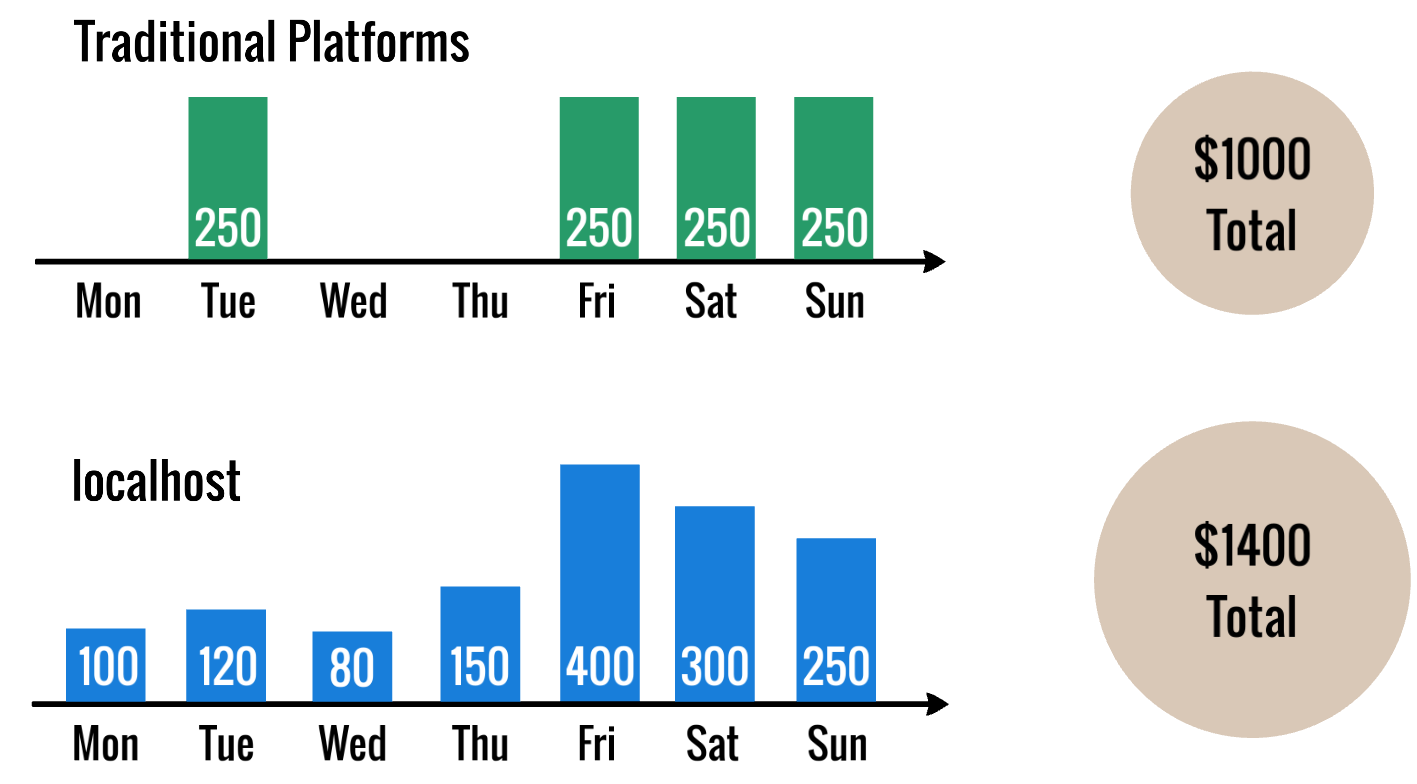
\includegraphics[width=\linewidth]{assets/fixedvsdynamic.png}
  \caption{Theoretical comparison of Fixed-Pricing vs Auctions}
  \label{fig:fixedVsDynamic}
\end{figure}

Figure~\ref{fig:fixedVsDynamic} shows theoretical earnings over the course of
a week for a traditional fixed-price platform and our \emph{localhost} platform.
Earnings are lower on the traditional platform as the price is deemed too steep
on days of low demand and the property is left empty.
By contrast, the \emph{localhost} allows income for hosts even on days of low demand,
albeit at a lower rate. On days with high demand, the price paid may exceed the
price that would have been statically set on traditional platforms. Guests also benefit
from this model as they can find bargains on days of low demand.

Due to the fast-paced nature of our auction system, our project focuses on
single night stays for guests.

\subsection{Concepts}

\subsubsection{Properties and Property Items}

As well as listing entire properties, hosts can choose to list individual rooms or
couches within a single property. These smaller listings within a property are
called property items, and are displayed on each property page. Each property item
has its own auction, thus a single property may have multiple auctions occurring
simultaneously.

\subsubsection{Auction Sessions}

\begin{table}[!h]
  \centering
  \begin{tabular}{|l|l|l|}
    \hline
    Session & Start Time & End Time \\ \hline
    1       & 12pm       & 6pm      \\
    2       & 6pm        & 8pm      \\
    3       & 8pm        & 10pm     \\
    4       & 10pm       & 12am     \\
    5       & 12am       & 3am      \\ \hline
  \end{tabular}
  \caption{Auction Session Times}
  \label{tab:sessionTimes}
\end{table}

Guests can book accommodation on \emph{localhost} by winning an auction.
Auctions on our platform run in fixed sessions ranging in time from two to six hours.
At the end of every session the highest bidder wins the auction and a booking is confirmed.
As seen in Table~\ref{tab:sessionTimes},
auction sessions start running from midday to 3am the following day, with shorter sessions
for stages of the day where a higher volume of bids are expected and longer sessions
for periods of low volume such as early afternoon.

The purpose of having multiple sessions is to give prospective guests multiple chances to
win a bid throughout the day. If the guest loses a bid earlier in the day, he has
additional chances later that night to win another bid. If auction
sessions were not enforced and owners could choose their own session times, they
would choose a single long session throughout the day which would
maximise the number of bids to optimise their profits.
Instead, hosts must decide which sessions their properties are listed for auction
based on personal factors such as the latest guest check-in time.

\subsubsection{Buyout Option}
A buyout option exists for guests to immediately purchase
the item without having to wait for the auction session to end. Guests may choose to
trade off cost for convenience and hosts receive large financial benefit from buyouts.
Buyouts will immediately end the auction session and award the property item to the buyer.

\subsubsection{Wallet}
A user must first deposit credit into their accounts before they can bid in auctions.
Once a bid is made in
an auction, the amount is immediately deducted from the wallet. This is to prevent
users from bidding on multiple properties and encourages users to commit to a single
property or room. Credits are immediately returned to the user's wallet if
he or she was outbid or the auction was bought out.
